\chapter{Miami Wealth, Credibility, and the Arithmetic of Getting to Yes}

This chapter follows a School of Hard Knocks interview, curated by LazyingArt LLC, and reads it as a lecture in commercial reasoning. We begin with yachts and spectacle, but the first mechanism the lecture really introduces is not money; it is permission. From there the argument unfolds in a tight order: credibility opens the door, scarcity hardens work into skill, sales becomes empathy, sacrifice prices the climb, risk is resized so that loss remains survivable, and finally value is priced in the buyer's own units. A short early stretch of the transcript is garbled and contributes no stable content, so we keep to the usable narrative line and mark approximate claims as approximate.

\section{Wealth Field and the Price of Access}

The lecture opens with quick cold approaches. A yacht appears, a stranger is stopped, the host announces ten million followers, and large money claims are thrown onto the page before any doctrine has been extracted from them. We should resist the temptation to treat this as mere showmanship. The lecture wants us to feel the gate before it gives us the key. In a private field, wealth is not first explained to us; it is first defended, and entry requires some credible signal.

Only then does the lecture widen the lens and tell us where we are. Miami is presented as a dense wealth field, and the opening arithmetic is scene-setting rather than census-like:
\begin{equation}
r_{\mathrm{Miami}} = 6,
\qquad
N_{\mathrm{billionaires}} > 12,
\qquad
F_{\mathrm{host}} = 10\times 10^{6}.
\end{equation}
Here \(r_{\mathrm{Miami}}\) is the host's stated national rank of Miami by millionaire count, \(N_{\mathrm{billionaires}}\) is the host's stated billionaire count, and \(F_{\mathrm{host}}\) is the follower base that functions as an access credential.

The cold open also throws down a few numerical fragments that are not yet explained. One speaker says he has made about \$300 million in a single year. Another fragment describes a company bought for \$25 million and sold for \$55 million three years later. We should not merge these into a single clean biography, but the second fragment does carry a simple piece of capital arithmetic:
\begin{align}
\Delta P
&= P_{\mathrm{sell}} - P_{\mathrm{buy}}
= \$55\,\mathrm{M} - \$25\,\mathrm{M}
= \$30\,\mathrm{M},\\
M_{\mathrm{exit}}
&= \frac{P_{\mathrm{sell}}}{P_{\mathrm{buy}}}
= \frac{55}{25}
= 2.2.
\end{align}
So even before the lecture settles on a full case study, it gives us a quick example of how wealth talk is often carried by rough multiples, gains, and exits.

What matters most in the opening, however, is not the size of the numbers but the recurring slogan that later becomes explicit: credibility matters. In this lecture, credibility is not an ornament. It is the condition under which suspicion softens, refusals become conversations, and the rest of the chapter can even begin.

\section{Lack, Early Labor, and Sales as Empathy}

After the opening spectacle the lecture drops down to ground level. The first substantial entrepreneur says she owns five businesses, that she first became an equity partner at twenty-four, and that she came from nothing: four children, a single mother, food stamps, and a trailer behind her grandparents' house. The register changes immediately. Wealth is no longer introduced as visible luxury but as a deliberate answer to lack.

The lecture then makes an important move. It does not leave lack as a motivational slogan. It turns lack into labor. At nine she starts working. By eighteen, while others are only beginning to think about work, she says she has already been at it for a decade. The point is not simply that she worked hard. The point is that early labor became usable capability. By the time she reached her first job out of college, she says she had both work ethic and sales expertise, and that combination let her outrun the people around her.

The host then asks the right question: what, exactly, is good selling? The answer is one of the clearest conceptual modules in the lecture. Selling is not pushing what we want to move. It is identifying the other person's problem, inhabiting it with them, speaking to the pain point in their language, and allowing trust to form before the solution is offered.

\paragraph{Sales Mechanism.}
A useful transcript-derived reconstruction is the following chain:
\begin{equation}
\text{problem} \to \text{empathy} \to \text{connection} \to \text{trust} \to \text{ask} \to \text{solution} \to \text{sale}.
\end{equation}
The order matters. If we begin with inventory, we stay on our side of the table. If we begin with the buyer's difficulty, the buyer begins to feel understood, and only then does the request for a solution become natural.

\begin{figure}
\centering
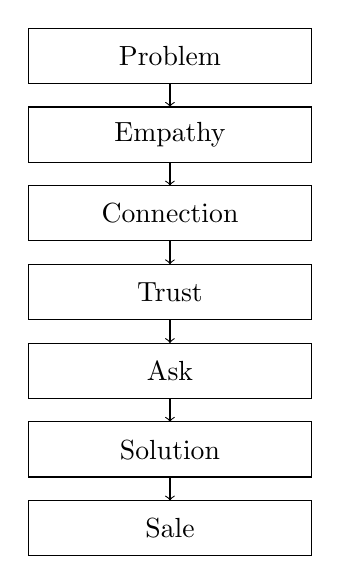
\begin{tikzpicture}[x=1cm,y=1cm]
\draw (0,0) rectangle (3.6,0.7);
\node at (1.8,0.35) {Problem};
\draw (0,-1.0) rectangle (3.6,-0.3);
\node at (1.8,-0.65) {Empathy};
\draw (0,-2.0) rectangle (3.6,-1.3);
\node at (1.8,-1.65) {Connection};
\draw (0,-3.0) rectangle (3.6,-2.3);
\node at (1.8,-2.65) {Trust};
\draw (0,-4.0) rectangle (3.6,-3.3);
\node at (1.8,-3.65) {Ask};
\draw (0,-5.0) rectangle (3.6,-4.3);
\node at (1.8,-4.65) {Solution};
\draw (0,-6.0) rectangle (3.6,-5.3);
\node at (1.8,-5.65) {Sale};
\draw[->] (1.8,0) -- (1.8,-0.3);
\draw[->] (1.8,-1.0) -- (1.8,-1.3);
\draw[->] (1.8,-2.0) -- (1.8,-2.3);
\draw[->] (1.8,-3.0) -- (1.8,-3.3);
\draw[->] (1.8,-4.0) -- (1.8,-4.3);
\draw[->] (1.8,-5.0) -- (1.8,-5.3);
\end{tikzpicture}
\caption{Transcript-derived editorial reconstruction of the lecture's sales path.}
\end{figure}

The lecture even gives the psychological marker of success. When the buyer thinks, ``This person gets my pain point,'' trust has already crossed the table.

\subsection{Question \& Answer}

Why does empathy sell better than product pushing?

Because the lecture does not treat a sale as the victory of pressure. It treats it as the transfer of trust after accurate diagnosis. If we begin with ``Here is what I want you to have,'' we are still speaking from our own inventory and our own urgency. If we begin by understanding how the other person got into difficulty, how that difficulty feels, and what would remove it, then the buyer begins to ask for help rather than defend against a pitch. In the lecture's logic, empathy is not softness. It is the shortest path to relevance.

\section{Sacrifice, Mobility, and Fearful Resistance}

Having shown us the advantage, the lecture now prices it. The same entrepreneur says that in her twenties she took no days off for four years, no vacations, while friends were marrying and having children. She moved from Boston to Saginaw, Michigan, a place described not as glamorous opportunity but as a hard piece of ground on which to make a name. The lecture is careful here. Credibility is not merely granted by an audience count or a logo. It is also built the slow way, by going where the work is and staying long enough for a reputation to harden.

Then comes the next correction. The lecture refuses the easy mythology of ``haters.'' Resistance does not always come from enemies. Sometimes it comes from those who love us and are afraid on our behalf. This matters because it changes the moral texture of the obstacle. The force opposing motion is not always malice; sometimes it is care that cannot imagine risk without catastrophe.

\subsection{Question \& Answer}

Are the people holding us back always enemies?

No. The lecture's answer is subtler. Loved ones may try to hold us in place not because they want our failure, but because they fear our exposure. That is why the response cannot be merely combative. We acknowledge the concern, we remain grateful, and we move anyway. The deep asymmetry in this part of the lecture is between borrowed fear and private judgment. Others may care, but they do not have direct access to the life we are trying to build.

This is an important beat in the chapter. Wealth is not opposed only by market difficulty. It is also opposed by social gravity. The lecture keeps that gravity intimate, which is precisely why it is powerful.

\section{Risk, Drawdown, Networking, and Speed}

The lecture then relocates to the Miami Beach Yacht Harbor, and again we are made to feel the gate: private docks, refusal at the entrance, the need to find an office, the slow pressure of working one's way in. This reset is not filler. It prepares the shift from bootstrap struggle to institutional scale.

Once on board, the hedge-fund operator gives a compact career arc: Wall Street, a firm later acquired by Bank of Montreal, a hedge fund, then a 2010 move from trading to execution inside a fintech company, followed eventually by a sale to a major Canadian bank. The lecture's point is not the romance of finance. It is the size and structure of the machine:
\begin{equation}
T_{\mathrm{fund}} \approx 28\,\mathrm{yr},
\qquad
N_{\mathrm{traders}} \approx 4000,
\qquad
N_{\mathrm{emp}} \approx 600,
\qquad
s_{\mathrm{mkt}} \approx 0.03\text{--}0.04.
\end{equation}
These are speaker-attributed scale markers. The exact denominator behind \(s_{\mathrm{mkt}}\) is not made precise in the transcript, but the strategic use of the number is clear: we are meant to see an operation with genuine market footprint.

Then comes the cleanest loss event in the lecture:
\begin{equation}
L_{\mathrm{day}} \gtrsim \$8\times 10^{6}.
\end{equation}
A little over \$8 million disappears in one day. The lecture does not linger on the melodrama of that fact. Instead it asks the right question: what rule survives the loss?

\begin{definition}
A risk choice is \emph{survivable} if a total loss of the position still leaves the investor or operator able to continue.
\end{definition}

If \(I\) denotes the capital placed at risk, the lecture's rule can be written in minimal form as
\begin{equation}
W_{\mathrm{after}} = W_{\mathrm{before}} - I,
\end{equation}
with \(I\) chosen so that \(W_{\mathrm{after}}\) is still a balance sheet we can inhabit even if the position goes to zero.

\subsection{Question \& Answer}

How much risk can we actually afford to take?

Not the amount that flatters confidence in the good state, but the amount that remains survivable in the bad one. The lecture's answer is austere and practical. We do not size exposure by mood. We size it by continuity. The point is not to avoid loss altogether. The point is to make sure that even a full loss does not remove us from the game.

The lecture then pivots from risk to relationships. The host observes that some very rich Wall Street figures became rich less by placing trades than by making deals. This is the cue for the next mechanism: networking. A golf-tournament contact is not allowed to cool. The partner is told to call immediately, the man comes in, sees something real, becomes chairman, and the company takes a step upward. The process is simple enough to write:
\begin{equation}
\text{contact} \to \text{immediate call} \to \text{meeting} \to \text{chairman role} \to \text{company pivot}.
\end{equation}
This is one of the lecture's cleanest lessons in timing. Recognition decays. Memory cools. Opportunity has a half-life. That is why speed matters.

The speaker then broadens speed into the language of mindset and manifesting. We need not inflate that vocabulary into a theorem it is not trying to be. In the lecture it means something concrete: imagine the objective, identify the steps, and move without delay. The mystical language sits on top of an operational rule.

\section{Credibility, Systems, and the Dollar Value of Time}

Before the next interview, the lecture inserts a brief operating aside. Companies, we are told, die from indigestion and starvation. The slogan is useful because it names two distinct failure modes. A company can die because it never secures enough business, but it can also die because growth outruns systems, inventory, accounting, and control. This aside is structurally important. It bridges the move from finance and networking to the next interview, where value will be priced in terms of operational acceleration.

Then the host approaches the next businessman and again deploys the same gate-opening tool: audience size. ``Credibility matters,'' he says. The line is repeated almost like an operator identity. Credibility does not guarantee substance, but it changes the initial condition of the interaction. A refusal becomes a minute of attention.

That minute yields one of the strongest business sequences in the lecture. The entrepreneur says he helps companies navigate regulatory and clinical pathways for products. Asked about the most common mistake business owners make, he answers: CEO ego. Asked about sales, he says he does not sell anything; he finds what the client needs and hits the client's goal. Only after those two pieces are in place does the lecture arrive at its sharpest arithmetic.

He says the company did, approximately, \$8.5 billion last year:
\begin{equation}
R_{\mathrm{company}} \approx \$8.5\times 10^{9}.
\end{equation}
That number is explicitly hedged in the transcript, and we should keep it that way. Its function is not to certify a balance sheet but to tell us that the later pricing example is being given by a person who thinks in operating scale.

Now the interview turns on one of its best pivots: not ``what does this cost?'', but ``what is this worth to you?'' Suppose, he says, that a product would do \$12 million in a year, and suppose he can bring it to market three months earlier.

\begin{proposition}
Under the lecture's linear-accrual heuristic, if a product would produce \(R_{\mathrm{year}} = \$12\,\mathrm{M}\) in a year and the launch is accelerated by \(\Delta t = 3\) months, then the gross incremental value created for the buyer is
\begin{equation}
\Delta V = R_{\mathrm{year}}\frac{\Delta t}{12} = \$3\,\mathrm{M}.
\end{equation}
\end{proposition}

\begin{proof}
We first compute the monthly revenue rate:
\begin{align}
R_{\mathrm{month}}
&= \frac{R_{\mathrm{year}}}{12}
= \frac{\$12\,\mathrm{M}}{12}
= \$1\,\mathrm{M/month}.
\end{align}
Three months of acceleration therefore add
\begin{align}
\Delta V
&= R_{\mathrm{month}}\Delta t
= (\$1\,\mathrm{M/month})(3\,\mathrm{months})
= \$3\,\mathrm{M}.
\end{align}
\end{proof}

The lecture then compares this gain to the fee:
\begin{align}
F &= \$300{,}000,\\
S_{\mathrm{buyer}} &= \Delta V - F = \$3{,}000{,}000 - \$300{,}000 = \$2{,}700{,}000,\\
\frac{\Delta V}{F} &= 10.
\end{align}
So the fee is one tenth of the gross incremental value created, and the buyer's gross surplus is \$2.7 million.

\subsection{Question \& Answer}

Why is a \$300{,}000 fee cheap if it creates \$3 million in value?

Because the lecture's pricing rule is buyer-side rather than seller-side. The relevant question is not how many hours the consultant worked, but how much value the client receives by moving earlier. Once the outcome is specified, price can be judged relative to that outcome. In this case, three months of earlier market entry on a \$12 million annual revenue stream produces a gross value of \$3 million. On that arithmetic, \$300{,}000 is not large.

A caution belongs here. This is deliberately rough business arithmetic. It does not include margins, adoption curves, cost of goods, or regulatory uncertainty. But the lecture is not trying to write a full discounted cash-flow model. It is trying to make one sharp point: time can be priced when time moves revenue.

The same interview closes with another claim that the lecture does not over-decorate. The entrepreneur says he has lost everything and rebuilt four times. When asked what the common factor is, he does not name a special product. He says the policies and procedures are the same: treat people right, do what they are looking for, and outwork everybody else. The objects change; the method remains invariant.

\section{Keeping the Machine Alive}

The final interview narrows the scale and, by narrowing it, grounds the chapter. A mechanical engineer says he owns a company, has been at it for twenty-two years, has not yet become a millionaire, but is trying to be. The host then asks the right operating questions: revenue, profit, scaling constraint, hiring, family, and downside. We are no longer in the territory of headline wealth. We are in the slower mathematics of keeping a business alive.

The company did about \$30 million in sales last year, with profit of roughly \$2 million to \$3 million. The lecture immediately interprets this not as leisurely abundance but as reinvestment pressure. Money is coming in, but much of it is going back into the machine:
\begin{equation}
R_{\mathrm{field}} \approx \$30\,\mathrm{M},
\qquad
\Pi_{\mathrm{field}} \approx \$2\text{--}3\,\mathrm{M}.
\end{equation}
The implied operating margin is therefore
\begin{equation}
m = \frac{\Pi_{\mathrm{field}}}{R_{\mathrm{field}}}
\approx \frac{2}{30}\text{--}\frac{3}{30}
\approx 0.067\text{--}0.10.
\end{equation}
So the lecture closes not with a fantasy of effortless owner extraction, but with a thinner operating spread and the need to keep building.

The stated bottleneck is labor. The company cannot scale without good employees, and good employees are hard to find. That fact is then nested inside a broader pattern: the most important hire so far is a twin brother; the father trained them into the business; physical discipline matters; up-and-down cycles are normal; and it is easier to spend into an expansion than to step back when the cycle contracts.

\subsection{Question \& Answer}

Why is keeping a company harder than starting one?

Because starting is an event, while keeping is a repeated negotiation with labor, standards, reinvestment, family, and appetite. The lecture's final owner describes this exactly. We must keep employees, keep the work quality up, keep our own lifestyle from ratcheting upward too far, and keep enough flexibility to survive a bad year. What is difficult is not merely ignition. It is sustained combustion.

This is also where the lecture makes a final distinction between entrepreneurship and employment. Not everyone, the speaker says, is built for entrepreneurship. Some people are great employees. The point is not to grade those lives morally. The point is to identify the structure of sacrifice. Entrepreneurship demands irregular pressure not only from the owner but from spouse, children, travel, routine, and tolerance for uncertainty.

\section{Summary}

The chapter begins with access because, in this lecture, access is the hidden first principle. Before we can talk about wealth, we have to get past the gate. From there the lecture moves deliberately: scarcity becomes labor, labor becomes sales skill, sales becomes empathy, empathy is priced by sacrifice, and only then do we rise into the larger scales of hedge funds, institutional deals, and billion-dollar revenue claims.

The later sections sharpen these themes into commercial arithmetic. Risk is not abolished; it is resized so that failure remains survivable. Networking is not social decoration; it is time-sensitive conversion of weak contact into strong leverage. Value pricing is not motivational rhetoric; it is the computation of what faster market entry is worth to the buyer. And the final operating case restores the earthly truth that a business may have meaningful revenue and still live inside labor shortages, reinvestment pressure, and cyclical strain.

What remains, when the spectacle falls away, is a sequence of local rules. Get into the room. Understand the other person's need. Risk only what can go to zero without taking us down with it. Move while the contact is still warm. Price time in the buyer's units. And do not confuse starting a machine with keeping it alive.